\documentclass[A4,12PT, english, twocolumn]{journal}
\usepackage{amsmath,amssymb,amsfonts}
\usepackage[margin=0.7in]{geometry}
\usepackage{graphicx}
\usepackage{enumitem}
\usepackage{xcolor}
\usepackage{hyperref}
\usepackage{tabularray}
\usepackage{multicol}
\usepackage{tikz}
\usepackage{circuitikz}
\usepackage{scalerel}
\usepackage{pict2e}
\usepackage{tkz-euclide}
\usetikzlibrary{calc}
\usetikzlibrary{patterns,arrows.meta}
\usetikzlibrary{shadows}
\usetikzlibrary{external}

%pgfplots
\usepackage{pgfplots}
\pgfplotsset{compat=newest}
\usepgfplotslibrary{statistics}
\usepgfplotslibrary{fillbetween}

\def\infinity{\rotatebox{90}{8}}

% Hiperlink
\hypersetup{
    colorlinks=true,
    linkcolor=blue,
    filecolor=magenta,      
    urlcolor=cyan,
    pdftitle={Overleaf Example},
    pdfpagemode=FullScreen,
}
%\usepackage{style}
\NewDocumentCommand{\Log}{o}{%
\IfNoValueTF{#1}{}{{}^{#1}\!}\log}%
  
%command buat logaritma dengan basisnya di pojok kiri
%\textheight=17cm
%\textwidth=10cm
%\usepackage{blindtext}
\setenumerate[1]{itemsep=0,5cm}
\setenumerate[2]{topsep=5pt, itemsep=5pt, label=\textbf{\Alph*}.}

\title{Matematika Saintek \& Fisika UTUL UGM 2019 Kode 624}
\author{Fauzan Akbar Sukandar Putra \\ \LaTeX}

\begin{document}

\maketitle

%\begin{minipage}{0.5\textwidth}
\begin{enumerate}
%1%
\item Banyaknya bilangan tiga digit yang disusun dari angka $0,1.2.3.4.5.6.7.8.9$ dengan syarat semua digitnya berbeda atau jika ada digit yang sama, letaknya tidak boleh berdekatan, adalah \dots
    \begin{enumerate}
        \item $576$ 
        \item $648$
        \item $729$
        \item $765$
        \item $810$
    \end{enumerate}
  
%2%
\item Jika $4^x+4^{-x}-2^{2-x}+2^{2+x}-7=0$, dengan $x>0$, maka $2^x+2^{-x}=\dots$
    \begin{enumerate}
        \item $\sqrt{2}$
        \item $\sqrt{5}$
        \item $\sqrt{7}$
        \item $\sqrt{10}$
        \item $\sqrt{11}$
    \end{enumerate}
     
%3%  
\item Jika $x>0$ dan $y>0$ memenuhi sistem persamaan:
\begin{center}
    \begin{cases}
        $3\left(x^2-1 \right)-2\left(y+1 \right)=-1$\\
        $-2\left(x-1 \right)+3\left(y+1 \right)=13$\\
    \end{cases}
\end{center}
maka nilai $x^2+y$ adalah \dots
    \begin{enumerate}
        \item $20$
        \item $16$
        \item $8$
        \item $6$
        \item $5$
    \end{enumerate}
   
%4%
\item $\lim\limits_{x \longrightarrow 0} {\frac{\sqrt{1-\cos 4x^2}}{1-\cos 2x}}=$ \dots
    \begin{enumerate}
        \item $1$
        \item $\sqrt{2}$
        \item $2$
        \item $2\sqrt{2}$
        \item $4$
    \end{enumerate}

%5%
\item Diketahui $a,\frac{1}{a},\frac{1}{a^2+2}. \; \; \; a\neq 0$. berturut-turut merupakan suke ke-$3, \; 4,$ dan ke-$5$ barisan geometri dengan rasio \\ $r \neq 1$. Hasil kali lima suku pertama barisan geometri tersebut adalah \dots
    \begin{enumerate}
        \item $42 \frac{5}{8}$
        \item $32 \frac{5}{8}$
        \item $32$
        \item $24 \frac{5}{8}$
        \item $24$
    \end{enumerate}
    
%6%
\item Diketahui vektor-vektor $\Vec{u} = \left(a,a+1,2 \right)$ dan $\Vec{v} = \left(1,1,1 \right)$. Jika vektor proyeksi $\Vec{u}$ pada $\Vec{v}$ adalah $\Vec{w} = \left(2,2,2 \right)$. Maka panjang vektor $\Vec{u}$ sama dengan \dots
    \begin{enumerate}
        \item $\frac{3}{2}$
        \item $\frac{5}{2}$
        \item $\frac{3}{2} \sqrt{2}$
        \item $\frac{5}{2} \sqrt{2}$
        \item $\frac{1}{2}$
    \end{enumerate}
    
%7%
\item Jika $x \in \left[-\frac {\pi}{6},0 \right]$, maka nilai minimum dari \\ $\cot \left( {x + \frac{\pi}{3}} \right) - \tan \left( {\frac{2\pi}{3}-x} \right)$ tercapai saat $x=$ \dots
    \begin{enumerate}
        \item $0$
        \item $-\frac{\pi}{12}$
        \item $-\frac{\pi}{9}$
        \item $-\frac{\pi}{8}$
        \item $-\frac{\pi}{6}$
    \end{enumerate}
    
%8% 
\item Diberikan bilangan real $a>0$ dan $a \neq 1$. Jika $^a\Log y, \; ^a\Log \left(y+1 \right), \; ^a\Log \left(3y+1 \right)$ membentuk tiga suku berurutan barisan aritmatika, maka kuadrat nilai-nilai $y$ yang mungkin adalah \dots
    \begin{enumerate}
        \item $\dfrac{1}{3}$
        \item $\dfrac{1}{2}$
        \item $1$
        \item $2$
        \item $3$
    \end{enumerate}
    
%9% 
\item Jika $^{a^2} \Log \left( 3^a-8 \right)^{-4} \cdot \; ^{3} \Log \sqrt{a} = a-2$. \\ maka $^a \Log \left( \frac{1}{8} \right) = $\dots
	\begin{enumerate}
		\item $0$
		\item $-1$
		\item $-2$
		\item $-3$
		\item $-4$
	\end{enumerate}
	
%10%
\item Diberikan kubus $ABCD.EFGH$. Jika $O$ titik tengah $DH$ dan $P$ adalah titik tengah $BF$. Maka perbandingan luas $\Delta AOP$ dan $\Delta AFC$ \dots
   \begin{enumerate}
        \item $1:2$
        \item $\sqrt{2}:1$
        \item $1:3$
        \item $2:1$
        \item $\sqrt{2}:2$
   \end{enumerate}
   
%11%
\item Misalkan $U_n$ menyatakan suku ke-$n$ dari barisan geometri. Jika $U_3-U_2 = 6$ dan $U_4-U_2 = 18$. Maka $U_5+U_3=$ \dots
    \begin{enumerate}
        \item $40$
        \item $50$
        \item $60$
        \item $70$
        \item $80$
    \end{enumerate}
  
%12%
\item Suku banyak $p(x)$ bersisa $2$ jika dibagi $x-1$ dan tak bersisa jika dibagi $x+1$. Suku banyak $q(x)$ bersisa $2x$ jika dibagi $x^2-1$. Jika suku banyak $p(x)+q(x)$ dibagi $x^2-1$, maka sisanya adalah \dots
    \begin{enumerate}
        \item $3x-1$
        \item $3x+1$
        \item $-3x+2$
        \item $-3x-2$
        \item $3x+2$
    \end{enumerate}
    
%13%
\item Bilangan $A>0$ sehingga lingkaran \\ $x^2+y^2+2x-4Ay+40=0$ mempunyai jari-jari $A+1$ adalah \dots
    \begin{enumerate}
        \item $5$
        \item $4$
        \item $3$
        \item $2$
        \item $1$
    \end{enumerate}

%14%
\item Banyaknya bilangan real $x$ yang memenuhi persamaan $\left|x^2-4 \right| = x+ \left|x-2 \right|$ adalah \dots
    \begin{enumerate}
        \item $0$
        \item $1$
        \item $2$
        \item $3$
        \item $4$
    \end{enumerate}

%15%
\item Jika garis singgung kurva $y=x^3-3x^2-9x$ di titik $\left(a,b \right)$ mempunyai gradien $15$. Maka nilai $a+b$ yang mungkin adalah \dots
\begin{enumerate}
       \item $0$
       \item $-2$
       \item $-4$
       \item $-6$
       \item $-8$
    \end{enumerate}
    

%FISIKA %
%16%
\newpage
\item Sebuah benda bergerak sepanjang garis lurus dengan kecepatan sebagai fungsi waktu diperlihatkan pada gambar. Berapakah kerja yang dilakukan oleh gaya yang bekerja pada benda itu sehingga benda mengalami gerak sebagaimana diperlihatkan dalam grafik itu dari $t=0 \, s$ sampai $t=7 \, s$?
\begin{center}
    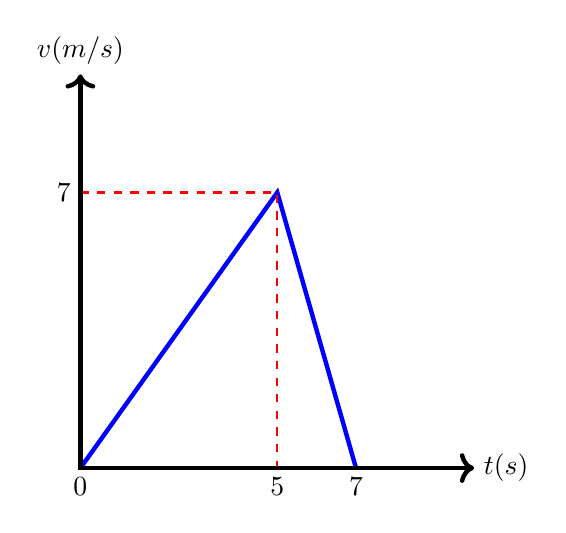
\begin{tikzpicture}[scale=0.5]
        %GRID
        %\draw[lightgray] (0,0) grid (10,10);

        %GRAFIK
        \draw[blue, ultra thick] (0,0) -- (5,7) -- (7,0);

        %GARIS BANTU
        \draw[dashed, red, thick] (0,7) -- (5,7) -- (5,0);

        %AXIX
        \draw[ultra thick, <->] (10,0) -- (0,0) -- (0,10);

        %LABEL
        \node[left] at (0,7){$7$};
        \node[below] at (5,0){$5$};
        \node[below] at (7,0){$7$};
        \node[below] at (0,0){$0$};
        \node[right] at (10,0){$t(s)$};
        \node[above] at (0,10){$v(m/s)$};
    \end{tikzpicture}
\end{center}
    \begin{enumerate}
        \item $0,0 \, J$
        \item $17,5 \, J$
        \item $24,5 \, J$
        \item $27,8 \, J$
        \item $28,5 \, J$
    \end{enumerate}
  
%17%
\item Panjang gelombang cahaya tampak memiliki kisaran panjang gelombang $380 \, nm$ - $700 \, nm$. Sebuah detektor cahaya yang menggunakan prinsip efek fotolistrik, agar dapat mendeteksi seluruh spektrum cahaya tampak, harus menggunakan metal dengan fungsi kerja maksimal \dots
    \begin{enumerate}
        \item $1,02 \, eV$
        \item $1,77 \, eV$
        \item $2,36 \, eV$
        \item $2,48 \, eV$
        \item $3,26 \, eV$
    \end{enumerate}
     
%18%
\item Tinjau suatu partikel yang ditembakan dengan kecepatan awal $v_0$ yang membentuk sudut $\theta$ terhadap arah horizontal. Jika partikel kedua dilempar dengan kecepatan yang sama dan dengan sudut $2\theta$, hitunglah perbandingan jarak horizontal maksimum partikel satu dan dua jika percepatan gravitasi adalah $g$!
    \begin{enumerate}
        \item $\cos{2\theta}$
        \item $2\cos{2\theta}$
        \item $1/(2\cos{2\theta})$
        \item $\sin{2\theta}$
        \item $1/(\sin{2\theta})$
    \end{enumerate}
   
%19%
\item Sebuah pegas memiliki konstanta pegas $k$, digantungkan pada sebuah papan pada arah vertikal. Sebuah bola bermassa $m$ diikatkan pada pegas yang tak direggangkan dan dibiarkan jatuh. Hitunglah jarak jatuhnya balok tersebut sebelum balok mulai bergerak balik jika diketahui percepatan gravitasi adalah $g$!
    \begin{enumerate}
        \item $2mg/k$
        \item $mg/k$
        \item $2mgk$
        \item $mk/g$
        \item $mk$
    \end{enumerate}

%20%
\item Seorang dengan massa $64 \, kg$ melakukan terjun bebas dengan lengan dan kaki terlentang sedemikian rupa sehingga mengalami hambatan udara dengan kecepatan terminal $180 \, km/jam$. Jika gaya hambat udara sebanding dengan $bv^2$ dengan $b$ adalah konstanta, dan percepatan gravitasi adalah $9,81 \, m/s^2$, hitunglah nilai konstanta $b$!
    \begin{enumerate}
        \item $1,5 \, kg/m$
        \item $1,0 \, kg/m$
        \item $0,5 \, kg/m$
        \item $0,25 \, kg/m$
        \item $0,125 \, kg/m$
    \end{enumerate}

%21%
\item Sebuah sumber bunyi menimbulkan taraf intensitas (TI) sebesar $10 \; dB$. Jika ada 10 sumber bunyi itu yang identik, berapakah taraf intersitasnya?
    \begin{enumerate}
        \item $100 \, dB$
        \item $40 \, dB$
        \item $30 \, dB$
        \item $20 \, dB$
        \item $11 \, dB$
    \end{enumerate}
    
%22%
\item Sebuah silinder berpiston berisi gas ideal yang volumenya $2 \; m^3$, tekanannya $10^5 \; Pa$ dan suhunya $300 \; K$. Silinder itu kemudian disentuhkan pada tandon kalor yang suhunya dijaga tetap pada $900 \; K$. Gas mengalami ekspansi pada tekanan tetap sehingga suhunya menjadi $900 \; K$. Berapakah volume gas ideal pada akhir proses ekspansi?
    \begin{enumerate}
        \item $6 \; m^3$
        \item $5 \; m^3$
        \item $4 \; m^3$
        \item $3 \; m^3$
        \item $2 \; m^3$
    \end{enumerate}
    
%23%
\item Suatu mesin melakukan kerja $200 \; J$ untuk setiap putaran. Jika panas yang terbuang adalah $400 \; J$ untuk setiap putaran mesin, maka efisiensi mesin tersebut adalah \dots
    \begin{enumerate}
        \item $1/4$
        \item $1/3$
        \item $2/3$
        \item $3/4$
        \item $1$
    \end{enumerate}
    
%24%
\item Terkait dengan medan magnet, manakah pernyataan berikut yang benar \dots
	\begin{enumerate}
		\item Garis-garis gaya medan magnet selalu berbentuk kurva tertutup
		\item Garis-garis gaya medan magnet dapat berbentuk kurva terbuka
		\item Garis-garis gaya medan magnet menuju ke satu titik yang sama
		\item Garis-garis gaya medan magnet meninggalkan satu titik yang sama
		\item Garis-garis gaya medan magnet bisa saling berpotongan
	\end{enumerate}
	
%25%
\item Tiga buah resistor, masing-masing sebesar $15\Omega, \; 4\Omega$ dan $8\Omega$ disambung secara seri kemudian dihubungkan dengan baterai dengan beda potensial $9 \; volt$. Perbandingan beda potensial yang terukur di ujung-ujung resistor $4\Omega$ dengan beda potensial totalnnya adalah \dots
   \begin{enumerate}
        \item $4/27$
        \item $8/27$
        \item $15/27$
        \item $19/27$
        \item $23/27$
   \end{enumerate}
   
%26%
\item Medan magnet pada jarak $10 \; cm$ dari suatu kawat berarus listrik $1 \; A$ adalah $2 \; \mu T$. Pada jarak sejauh $1 \; cm$ dari kawat, medan magnetnya menjadi \dots
    \begin{enumerate}
        \item $200 \; \mu T$
        \item $20 \; \mu T$
        \item $2 \; \mu T$
        \item $0,2 \; \mu T$
        \item $0,02 \; \mu T$
    \end{enumerate}
  
%27%
\item Seutas kawat yang panjangnya $0,2 \; m$ bergerak dengan kecepatan $1,5 \; m/s$ sejajar medan magnet seragam dengan kekuatan $0,5 \; tesla$. besar ggl yang terinduksi di dalam kawat tersebut adalah \dots
    \begin{enumerate}
        \item $3 \; volt$
        \item $2,25 \; volt$
        \item $1 \; volt$
        \item $0,6 \; volt$
        \item $0 \; volt$
    \end{enumerate}
    
%28%  
\item Seberkas cahaya datang sejajar sumbu utama sebuah lensa cembung sehingga dibiaskan mengumpul di titik apinya. Jika di depan lensa cembung itu diletakkan lensa cembung kedua, maka \dots
    \begin{enumerate}
        \item Berkas dibiaskan dan mengumpul di titik yang lebih jauh
        \item Berkas dibiaskan dan mengumpul di titik yang lebih dekat
        \item Berkas dibiaskan dan mengumpul di titik api lensa pertama
        \item Berkas dibiaskan dan mengumpul di titik api lensa kedua
        \item Berkas dibiaskan menyebar
    \end{enumerate}

%29%
\item Sebuah eksperimen interferensi Young dilakukan dengan menggunakan sinar laser Argon $(\lambda=515 \; nm)$. Jarak pisah antar celah adalah $0,5 \; nm$, dan pola interferensi nampak pada layar yang jaraknya $3,3 \, m$. Berapakah jarak antara pola terang yang berdekatan?
    \begin{enumerate}
        \item $1,7 \; mm$
        \item $3,4 \; mm$
        \item $5,1 \; mm$
        \item $6,8 \; mm$
        \item $7,2 \; mm$
    \end{enumerate}

%30%
\item Panjang lintasan optik bagi seberkas cahaya adalah perkalian antara panjang lintasan dalam medium dan indeks bias medium. Lintasan dari beberapa medium yang ditempuh dengan waktu paling singkat berarti \dots
    \begin{enumerate}
        \item Sebuah garis lurus
        \item Lintasan optik paling pendek
        \item Lintasan paling pendek dalam medium
        \item Tunduk pada hukum Lambert
        \item Membelok sesuai dengan frekuensi
    \end{enumerate}

%31%
\item Seseorang melihat benda yang terletak di suatu tempat dengan jelas. Tiba-tiba ia meletakkan lensa cembung tepat di depan matanya, sehingga benda itu terlihat kabur olehnya. Mengapa?
    \begin{enumerate}
        \item Bayangan bergeser ke belakang retina dan terbalik
        \item Bayangan bergeser ke belakang retina dan tegak
        \item Bayangan bergeser ke depan retina dan terbalik
        \item Bayangan bergeser ke depan retina dan tegak
        \item Bayangan tetap berada di retina dan tegak
    \end{enumerate}

%32%
\item Seorang pengamat bergerak dengan kecepatan $0,6 \; c$ menyusur permukaan bumi, dengan $c$ adalah cepat rambat cahaya dalam ruang hampa. Pengamat itu melewati subuah bangun di bumi yang terlihat olehnya sebagai sebuah lingkaran dengan jari-jari $1 \; m$. Bangun geometris itu jika dilihat oleh orang yang diam di bumi berupa elips dengan setengah sumbu pendek \dots
    \begin{enumerate}
        \item $0,80 \; m$
        \item $1,00 \; m$
        \item $1,25 \; m$
        \item $1,32 \; m$
        \item $1,36 \; m$
    \end{enumerate}

%33%
\item Relasi ketidakpastian Heisenberg bermakna bahwa \dots
    \begin{enumerate}
        \item Posisi dan momentum partikel tidak dapat diukur dengan pasti
        \item Posisi dan momentum partikel tidak dapat diukur dengan pasti secara simultan
        \item Posisi dan momentum partikel tidak dapat diukur secara simultan
        \item Posisi dan momentum partikel dapat diukur secara simultan dengan pasti
        \item Ketidakpastian pengukuran momentum dan posisi saling bebas
    \end{enumerate}

%34%
\item Elektron pada keadaan $6f$ pada atom hidrogen memiliki energi dan momentum sudut sebesar \dots
    \begin{enumerate}
        \item $E=-0,85 \, eV, \; L=\sqrt{6} \, h$
        \item $E=-0,54 \, eV, \; L=\sqrt{6} \, h$
        \item $E=-0,54 \, eV, \; L=\sqrt{12} \, h$
        \item $E=-0,38 \, eV, \; L=\sqrt{6} \, h$
        \item $E=-0,38 \, eV, \; L=\sqrt{12} \, h$
    \end{enumerate}

%35%
\item Energi ionisasi dari atom Hidrogen adalah $13,6 \; eV$. Berapakah energi dari tingkat keadaan $n=5$?
    \begin{enumerate}
        \item $2,72 \; eV$
        \item $-2,72 \; eV$
        \item $0,544 \; eV$
        \item $-0,544 \; eV$
        \item $0,628 \; eV$
    \end{enumerate}

\end{enumerate}
\end{document}  
